\documentclass[border=0.5pt]{standalone}
\usepackage{tikz}
\usepackage{amsmath}
\usepackage{sansmath}
\renewcommand{\familydefault}{\sfdefault}
\usetikzlibrary{arrows.meta,calc}
% ---------- colours ----------
\definecolor{cLP}{HTML}{2A78D6}   % CMH-LP
\definecolor{cHP}{HTML}{E34948}   % CMH-HP
\definecolor{cDB}{HTML}{1B9E8A}   % DBCCA
\definecolor{cBI}{HTML}{D08C1F}   % ISIMIP3BASD
\definecolor{cSR}{HTML}{7B5EA7}   % SRDRN-QDM
\definecolor{ink}{HTML}{1F2328}
\definecolor{mut}{HTML}{737B87}
\definecolor{lin}{HTML}{C9CED6}
\begin{document}
\sansmath
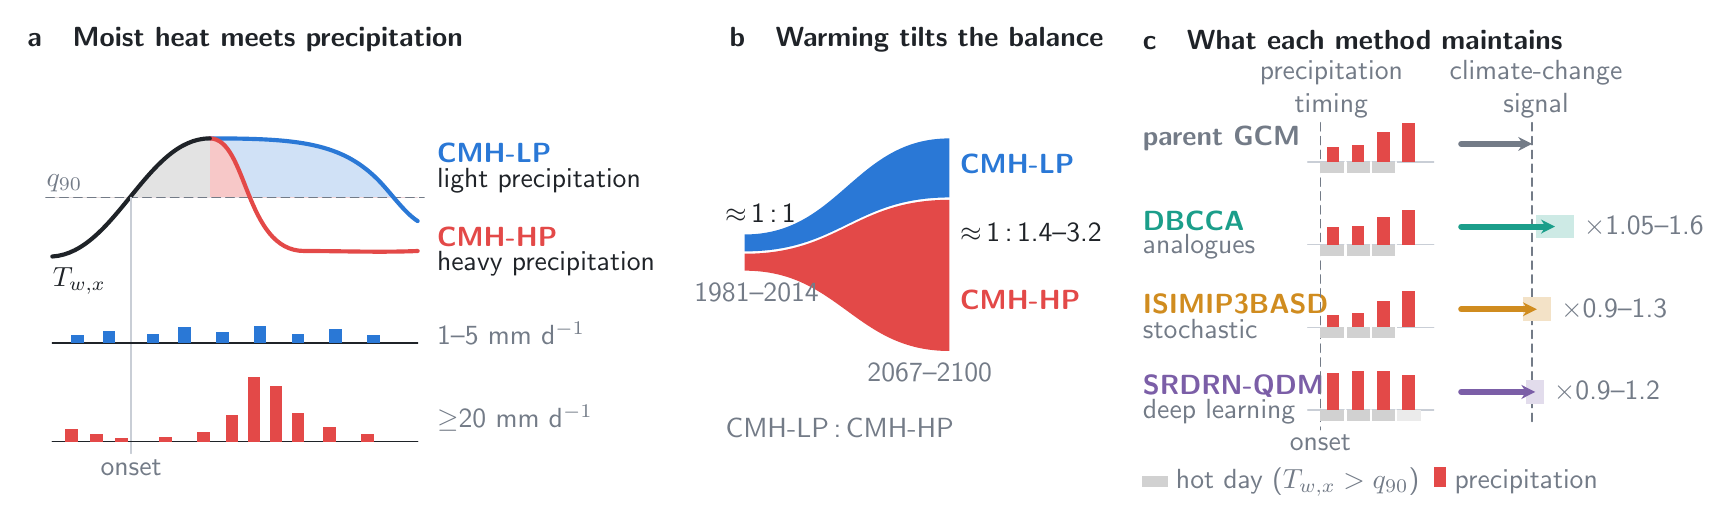
\begin{tikzpicture}[font=\sffamily\normalsize, text=ink, line cap=round, line join=round,
  ttl/.style={font=\sffamily\bfseries\normalsize, anchor=west, inner sep=0pt},
  lbl/.style={font=\sffamily\normalsize, inner sep=0pt},
  note/.style={font=\sffamily\normalsize, text=mut, inner sep=0pt}]

% =====================================================================
% (a) one onset, two endings
% =====================================================================
\node[ttl] at (0,6.3) {a\quad Moist heat meets precipitation};
\begin{scope}[xscale=.8]
\def\trunk{(0.4,3.55) .. controls (1.4,3.6) and (1.9,5.05) .. (2.9,5.05)}
\def\blue{.. controls (4.3,5.05) and (5.0,5.0) .. (5.6,4.5) .. controls (5.8,4.33) and (6.0,4.1) .. (6.2,4.0)}
\def\red{.. controls (3.5,5.05) and (3.45,3.62) .. (4.4,3.62) .. controls (5.0,3.62) and (5.6,3.6) .. (6.2,3.62)}
\begin{scope}\clip (0.3,4.3) rectangle (6.4,5.6);
  \fill[cLP!22] \trunk \blue -- (6.2,4.3) -- (0.4,4.3) -- cycle;
  \fill[cHP!30] \trunk \red -- (6.2,4.3) -- (0.4,4.3) -- cycle;
  \fill[black!11] \trunk -- (2.9,4.3) -- (0.4,4.3) -- cycle;
\end{scope}
\draw[mut, densely dashed, line width=.6pt] (0.3,4.3) -- (6.3,4.3);
\node[note, anchor=south west] at (0.3,4.36) {$q_{90}$};
\draw[cLP, line width=1.5pt] (2.9,5.05) \blue;
\draw[cHP, line width=1.5pt] (2.9,5.05) \red;
\draw[ink, line width=1.5pt] \trunk;
\node[note, anchor=north west, text=ink] at (0.4,3.42) {$T_{w,x}$};
\draw[lin, line width=.6pt] (1.65,4.3) -- (1.65,1.05);
\node[note, anchor=north] at (1.65,.98) {onset};
\draw[ink, line width=.5pt] (0.4,2.45) -- (6.2,2.45);
\foreach \x/\h in {.8/.10, 1.3/.16, 2.0/.12, 2.5/.2, 3.1/.14, 3.7/.22, 4.3/.12, 4.9/.18, 5.5/.1} {\fill[cLP] (\x-.1,2.45) rectangle (\x+.1,2.45+\h);}
\draw[ink, line width=.5pt] (0.4,1.2) -- (6.2,1.2);
\foreach \x/\h in {.7/.16, 1.1/.1, 1.5/.05, 2.2/.06, 2.8/.12, 3.25/.34, 3.6/.82, 3.95/.7, 4.3/.36, 4.8/.18, 5.4/.1} {\fill[cHP] (\x-.1,1.2) rectangle (\x+.1,1.2+\h);}
\node[lbl, anchor=west, text=cLP] at (6.5,4.86) {\textbf{CMH-LP}};
\node[note, anchor=west, text=ink] at (6.5,4.52) {light precipitation};
\node[lbl, anchor=west, text=cHP] at (6.5,3.8) {\textbf{CMH-HP}};
\node[note, anchor=west, text=ink] at (6.5,3.46) {heavy precipitation};
\node[note, anchor=west] at (6.5,2.58) {1--5 mm d$^{-1}$};
\node[note, anchor=west] at (6.5,1.5) {$\geq$20 mm d$^{-1}$};
\end{scope}

% =====================================================================
% (b) the balance shifts
% =====================================================================
\begin{scope}[xshift=28.84pt]
\node[ttl] at (7.9,6.3) {b\quad Warming tilts the balance};
\begin{scope}[xshift=-1.5cm]
\fill[cLP] (9.6,3.83) .. controls (10.8,3.83) and (11.0,5.05) .. (12.2,5.05) -- (12.2,4.3) .. controls (11.0,4.3) and (10.8,3.615) .. (9.6,3.615) -- cycle;
\fill[cHP] (9.6,3.585) .. controls (10.8,3.585) and (11.0,4.27) .. (12.2,4.27) -- (12.2,2.35) .. controls (11.0,2.35) and (10.8,3.37) .. (9.6,3.37) -- cycle;
\node[lbl, anchor=west, text=cLP] at (12.33,4.72) {\textbf{CMH-LP}};
\node[lbl, anchor=west, text=cHP] at (12.33,3.0) {\textbf{CMH-HP}};
\node[note, anchor=north] at (9.75,3.22) {1981--2014};
\node[note, anchor=north] at (11.95,2.2) {2067--2100};
\node[lbl, anchor=south] at (9.8,3.98) {$\approx$\,1\,:\,1};
\node[lbl, anchor=west] at (12.33,3.86) {$\approx$\,1\,:\,1.4--3.2};
\node[note, anchor=north west, align=left] at (9.35,1.5) {CMH-LP\,:\,CMH-HP};
\end{scope}
\end{scope}

% =====================================================================
% (c) what each of the three methods maintains
% =====================================================================
\begin{scope}[xshift=37.37pt]
\node[ttl] at (12.85,6.3) {c\quad What each method maintains};
\begin{scope}[xshift=-1.4cm]
\def\IX{17.15}   % centre of the timing icons
\def\AX{18.30}   % start of the change arrows (GCM change = 0.9 units -> tip at 19.20)
\def\dw{.32}     % width of one day; centre of day d at \IX + (d-1.5)*\dw, day 0 = onset (as in Fig. 4)
\def\ps{.0294}   % bar height per mm/d (common scale: 17 mm/d = 0.5)
\node[note, anchor=south, align=center] at (\IX-0.5,5.3) {precipitation\\timing};
\node[note, anchor=south, align=center] at (19.25,5.3) {climate-change\\signal};

\newcommand{\tpicon}[3]{%
  \draw[lin, line width=.5pt] (\IX-.8,#1) -- (\IX+.8,#1);
  \foreach \g [count=\d from 0] in {#2} {\ifnum\g>0 \fill[black!\g] ({\IX+(\d-2)*\dw},{#1-.14}) rectangle ({\IX+(\d-1)*\dw},#1);\fi}
  \foreach \k in {-1,0,1} {\draw[white, line width=.8pt] ({\IX+\k*\dw},{#1-.14}) -- ({\IX+\k*\dw},#1);}
  \foreach \d/\v in {#3} {\fill[cHP] ({\IX+(\d-1.5)*\dw-.08},#1) rectangle ({\IX+(\d-1.5)*\dw+.08},{#1+\v*\ps});}}
% --- row labels ---
\foreach \y/\n/\s/\c in {4.75/{parent GCM}/{}/mut, 3.70/{DBCCA}/{analogues}/cDB,
                         2.65/{ISIMIP3BASD}/{stochastic}/cBI, 1.60/{SRDRN-QDM}/{deep learning}/cSR} {
  \node[lbl, anchor=west, text=\c] at (14.25,\y+.30) {\textbf{\n}};
  \node[note, anchor=west] at (14.25,\y-.02) {\s};}
% --- onset guide ---
\draw[mut, densely dashed, line width=.5pt] ({\IX-2*\dw},5.25) -- ({\IX-2*\dw},1.35);
\node[note, anchor=north] at ({\IX-2*\dw},1.30) {onset};
% --- icons, days 0..+3 (T_wx - q90 on day +3: -0.45, -0.35, -0.42, -0.06) ---
\tpicon{4.75}{18,18,18,0}{0/6.59, 1/7.32, 2/13.06, 3/16.91}     % parent GCM
\tpicon{3.70}{18,18,18,0}{0/7.44, 1/8.27, 2/11.75, 3/14.83}     % DBCCA
\tpicon{2.65}{18,18,18,0}{0/5.39, 1/6.15, 2/11.50, 3/15.66}     % ISIMIP3BASD
\tpicon{1.60}{18,18,18,8}{0/15.82, 1/16.77, 2/16.74, 3/15.05}   % SRDRN-QDM
% --- key ---
\fill[black!18] (14.25,.62) rectangle (14.57,.76);
\node[note, anchor=west] at (14.67,.69) {hot day ($T_{w,x}>q_{90}$)};
\fill[cHP] (17.95,.62) rectangle (18.11,.88);
\node[note, anchor=west] at (18.21,.69) {precipitation};
% --- change arrows: GCM length is the reference; band = range of the amplification factor ---
\draw[mut, densely dashed, line width=.5pt] (19.20,5.25) -- (19.20,1.45);
\draw[-{Stealth[length=5pt,width=5pt]}, mut, line width=2.2pt] (\AX,4.98) -- (19.20,4.98);
% DBCCA  x1.05-1.59
\fill[cDB!22] (19.245,3.78) rectangle (19.731,4.08);
\draw[-{Stealth[length=5pt,width=5pt]}, cDB, line width=2.2pt] (\AX,3.93) -- (19.49,3.93);
\node[note, anchor=west] at (19.85,3.93) {$\times$1.05--1.6};
% ISIMIP3BASD  x0.87-1.27
\fill[cBI!25] (19.083,2.73) rectangle (19.443,3.03);
\draw[-{Stealth[length=5pt,width=5pt]}, cBI, line width=2.2pt] (\AX,2.88) -- (19.26,2.88);
\node[note, anchor=west] at (19.56,2.88) {$\times$0.9--1.3};
% SRDRN-QDM  x0.91-1.17
\fill[cSR!22] (19.119,1.68) rectangle (19.353,1.98);
\draw[-{Stealth[length=5pt,width=5pt]}, cSR, line width=2.2pt] (\AX,1.83) -- (19.24,1.83);
\node[note, anchor=west] at (19.47,1.83) {$\times$0.9--1.2};
\end{scope}
\end{scope}
\end{tikzpicture}
\end{document}